\documentclass[sw]{iosart2c}
\usepackage[utf8]{inputenc}
\usepackage[T1]{fontenc}
\usepackage{times}
\usepackage{natbib}
\usepackage{amsmath}
\usepackage{dcolumn}
\usepackage{graphicx}
\usepackage{url}
\usepackage{xspace}
\usepackage{color}
\usepackage{eurosym}
\usepackage{todonotes}
\usepackage[breaklinks]{hyperref}

\def\sectionautorefname{Section}
\def\subsectionautorefname{Section}

\usepackage{multirow}
\usepackage{booktabs}
\usepackage{tabularx}
\usepackage{array}
\usepackage{textcomp}

\newcolumntype{R}{>{\raggedleft\arraybackslash}X}
\newcolumntype{L}{>{\raggedright\arraybackslash}X}
\newcolumntype{C}{>{\centering\arraybackslash}X}

\newcommand{\TODO}[1]{{\color{red}{\textbf{TODO: {#1}}\xspace}}}
\newcommand{\CONSIDER}[1]{{\color{blue}{\textbf{CONSIDER: {#1}}\xspace}}}
\newcolumntype{d}[1]{D{.}{.}{#1}}

\newcommand{\claus}[1]{\todo[inline]{[Claus: #1]}}
%\newcommand{\textrdf}[1]{\texttt{#1}}
\newcommand{\vocab}[1]{\emph{#1}}

\usepackage[scaled]{beramono}
\newcommand\Small{\fontsize{9}{9.2}\selectfont}

\usepackage{listings}
%\lstset{language=Python}
%\lstset{%
% morekeywords={Create,View,As,Construct,With,From}
%}%
\lstset{emph={%  
    Create,View,As,Construct,With,From%
    },emphstyle={\color{blue}\bfseries}%
}%
\lstset{%
    numberbychapter=false,
    numbers=left,
    numberstyle=\tiny,
%    basicstyle=\footnotesize\ttfamily,
    basicstyle=\ttfamily \tiny,
    tabsize=2,
    framexleftmargin=2pt,
    captionpos=b,
    frame=single,
    breaklines=true
}
\lstdefinestyle{rdf}{numberblanklines=true, morekeywords={}}
\lstdefinestyle{sparql}{basicstyle=\ttfamily\scriptsize,numberblanklines=true,
    morekeywords={SELECT,OPTIONAL,FROM,DISTINCT,a,WHERE,FILTER,GROUP,ORDER,LIMIT,BY,IN,AS},
    emph={r,pub,aairObject,verb,person,bday,s,p,o},emphstyle=\textit
}
\lstdefinestyle{turtle}{basicstyle=\ttfamily\tiny ,numberblanklines=true,
    morekeywords={a, @prefix},
    morecomment=[s][\textrm]{<}{>},
    morecomment=[s][\textit]{"}{"},
}

% Default \todo{} to inline mode
\newcommand*{\origtodo}{}
\let\origtodo\todo
\renewcommand*{\todo}{\origtodo[inline]}

\firstpage{1} \lastpage{5} \volume{1} \pubyear{2012}
\begin{document}
\begin{frontmatter} 
\title{Countering language attrition with PanLex and the Web of Data}
\runningtitle{Countering language attrition with PanLex and the Web of Data}

\review{Name Surname, University, Country}{Name Surname, University, Country}{Name Surname, University, Country}

\author[A]{\fnms{Patrick} \snm{Westphal}},
\author[A]{\fnms{Claus} \snm{Stadler}},
\author[B]{\fnms{Jonathan} \snm{Pool}}
\address[A]{University of Leipzig, \{pwestphal, cstadler\}@informatik.uni-leipzig.de}
\address[B]{The Long Now Foundation, San Francisco, pool@panlex.org}

%(%!TEX TS-program = xelatex)
%(%!TEX encoding = UTF-8 Unicode)

\begin{abstract}
The world is losing some of its 7,000 languages.
Hypothesizing that language attrition might subside if all languages were inter\-trans\-latable, the PanLex project supports panlingual lexical translation by integrating all known lexical translations.
Semantic Web technologies can flexibly represent and reason with the content of its database and interlink it with linguistic and other resources and annotations.
%Using Semantic Web technologies can support achieving this goal, especially due
% to inference capabilities and the interlinking of the PanLex data with other data sources.
Conversely, PanLex, with its collection of translation links between more than a billion pairs of lexemes from more than 9,000 language varieties, can improve the coverage of the Linguistic Web of Data.
We detail how we transformed the content of the PanLex database to RDF, established conformance with the lemon and GOLD data models,
interlinked it with Lexvo and DBpedia, and published it as Linked Data and via SPARQL.
\end{abstract}

\begin{keyword}
Multilingual Linked Open Data, LLOD Cloud, PanLex, Lexical Resource, RDF, RDB2RDF, SPARQL, Sparqlify
\end{keyword}
\end{frontmatter}

\section{Introduction}
\label{sec:intro}
There are about 7,000 living languages\footnote{\url{http://www-01.sil.org/iso639-3/iso-639-3.tab}}, but language attrition has extinguished or threatened from 10\% to over 75\% of all languages in the last 60 years in various regions~\cite{lang_crisis}.
This attrition arguably imperils human biological knowledge and species diversity~\cite{nettle}. Hypothetically, panlingual intertranslatability would make all languages more useful and incentivize their preservation and revitalization. 

The PanLex project is making all languages' lexicons intertranslatable. In some contexts (e.g., profiles, catalogs, tags, search, and web navigation), lexical translation can be most of the translation load. PanLex systematically integrates lexical translations, found in diverse sources, into a database for research, applications, and public use. The content can be interpreted as a graph linking lexemes in ``is-a-translation-of'' relations, and permitting automated inference to additional, unattested relations.
%It documents the known lexical translations (translations of lexemes) among all
%languages.

The Semantic Web initiative has led to the development of standards and technologies
supporting a machine-readable and \mbox{-i}nter\-pretable Linked Data
network, known as the \emph{Web of Data}.\footnote{\url{http://www.w3.org/standards/semanticweb/}} From these efforts the \emph{Linked Open Data (LOD) cloud}\footnote{\url{http://lod-cloud.net/}} emerged.
%Technologies that support this aim are already available and in use in the so
%called \emph{Web of Data}.
A growing community is leveraging Semantic Web technologies for linguistic knowledge, building a \emph{Linguistic LOD (LLOD) cloud}.

%Whenever there is Linked Data making use of descriptions, such as labels, in any language with lexemes in citation form (lemmas), the data are potentially linkable to, and through, PanLex.
Here we describe how we connected PanLex to this Linked Data network.
In \autoref{sec:triplificate} we introduce the dataset, present a
PanLex RDF vocabulary, and explain how we transformed the one into the other and established conformance with additional data models.
\autoref{sec:linking} shows how we linked to other datasets of the LLOD cloud,
and \autoref{sec:publishing} is about the publication of the dataset.
Usage scenarios are given in \autoref{sec:usage}, and related work is discussed in \autoref{sec:related}.
Finally, \autoref{sec:conclusion} concludes paper.
%In \autoref{sec:related} we discuss related work, and, finally, in \autoref{sec:conclusion}, we
% summarize our recent and contemplated work.
%conclude 

\section{Triplification of the Raw Data}
\label{sec:triplificate}
In this section, we analyze the PanLex dataset; introduce our URI and vocabulary design, which resemble PanLex's conceptual model;
%, which was developed independently from other ontology engineering approaches.
summarize how we classified PanLex's instance data with additional data models; and explain our transformation of the data to RDF.

%As PanLex defines its own  conceptual model 

\subsection{Analysis of the Original Dataset}
\label{sec:analysis}
The PanLex \emph{database} is created by editors who consult \emph{information sources}\footnote{\url{http://panlex.org/tech/plrefs.shtml}}, such as mono- and multilingual dictionaries, glossaries, standards, and thesauri. The data include single- and multi-word expressions, corresponding meanings assigned to them, and related information.
%While copies of the sources would not be interoperable,
PanLex data constitute editors' \emph{interpretations} of sources' \emph{assertions} that two or more \emph{expressions} share a \emph{meaning}\footnote{\url{http://panlex.org/tech/doc/design/panlex-db-design.pdf}}.
The most important entities and relations of PanLex's conceptual model are depicted in \autoref{fig:db-schema}.

\begin{figure}
  \centering
  \includegraphics[width=0.42\textwidth]{images/schema_new.png}
  \caption{The PanLex database schema}
  \label{fig:db-schema}
\end{figure}

\begin{itemize}
  \item The \emph{source} entity is the authority to which an editor attributes assertions about lexical translations.
  \item \emph{Expressions} are lexical entities, each uniquely identified with a text, i.e. a string of (Unicode) characters, and a variety of a language. Expressions resemble lemmas or dictionary-entry headwords, but differ from them in at least two ways. (1) Homographs, such as the verb ``hide'' (conceal) and the noun ``hide'' (animal skin) in English, are treated as a single expression in PanLex. (2) Multiword expressions, such as ``fall in love'', traditionally found in an entry headed by one of their words, such as ``fall'' or ``love'', are treated as independent expressions in PanLex.
%Expression texts are constrained to comply with Unicode Normalization Form NFC.
% ~Claus: If we state this, we also have to cite NFC, which requires again more space
    \item \emph{Languages} in PanLex are identified using ISO 639-3\footnote{\url{http://www.sil.org/iso639-3/codes.asp}} individual and macrolanguage codes, ISO 639-2\footnote{\url{http://www.loc.gov/standards/iso639-2/}} collective codes, and ISO 639-5\footnote{\url{http://www.loc.gov/standards/iso639-5/}} codes.
    \item \emph {Language varieties} are collections of expressions. Each has a unique identifier: a language code and a distinguishing integer. For example, six dialects of Ahtna are identified as ``aht-000'' through ``aht-005''. These labels are, themselves, treated as a (controlled) language variety, whose expressions (i.e. the labels) are translated into natural languages and other controlled languages (such as the IETF standard BCP 47\footnote{\url{http://tools.ietf.org/html/bcp47}}).
%The only properties of this entity are ambiguity and synonymy: Controlled language varieties are usually defined to prohibit both of these.
    \item \emph{Meanings} are entities assigned to expressions, thereby identifying expressions as translations or synonyms. For example, a source's translation of the German expression ``klingen'' into English as ``ring, sound, seem'' can be interpreted as (1) the assignment of a single meaning to all four expressions or (2) the assignment of two or three meanings to ``klingen'' and of one of those to each of the English expressions. Meanings are source-specific. The identification and consolidation of equivalent meanings of distinct sources is a research topic, not a database feature. Meanings can have properties of three types. (1) \emph{Definitions} are descriptions of a meaning, consisting of text strings annotated as being in particular language varieties. (2) \emph{Domains} are expressions (e.g., ``medicine'') that characterize a meaning, but do not express it. (3) \emph{Meaning identifiers} are strings acting as references to identifiers in a source.
    \item \emph{Denotations} are assignments of meanings to expressions. A denotation may have one or more \emph{word classes} (a closed set based on OLIF, the Open Lexicon Interchange Format) and/or \emph{metadata} (arbitrary strings paired as keys and values).
    %For example, \emph{fall} can be a verb or a noun for autumn.
    %Homonyms are those expressions that are connected to multiple meanings.
  \item \emph{Users} may define sources, attribute data to them, and define language varieties.
  \item Among the properties of sources are \emph{licenses}. Some of the license categories are \emph{public domain},
%\emph{Creative Commons (CC)},
\emph{request} (author invites inquiries),
%\emph{GNU General Public License (GPL)},
%\emph{GNU Lesser General Public License (LGPL)},
\emph{GNU Free Documentation License (FDL)},
%\emph{MIT License}, \emph{copyright} (without a more liberal license),
and \emph{PanLex Use Permission} (specific permission for use in PanLex).
    The distribution of licenses is shown in \autoref{tbl:plx-license-counts}.
%as of January 2014
\end{itemize}

\begin{table}
\centering
\begin{scriptsize}
\begin{tabular}{lrclrclr}
License          & Count &&
License          & Count &&
License          & Count \\
\cline{1-2} \cline{4-5} \cline{7-8}
\emph{copyright} &  1343  && \emph{LGPL}      &     9 && \emph{PD}           & 149 \\
\emph{CC}          &   387   && \emph{MIT}         &    32 && \emph{other}       &   106 \\
\emph{FDL}        &    24    && \emph{PanLex}    &    7 && \emph{unknown}  &  1958 \\
\emph{GPL}        &   172   && \emph{request}    &     5 \\
\end{tabular}
\end{scriptsize}
\caption{Number of sources using a certain license}
\label{tbl:plx-license-counts}
\end{table}

\autoref{fig:plx-entity-counts} gives entity counts as of January 2014.
\begin{table}
  \centering\begin{scriptsize}
  \begin{tabular}{lrclr}
    Entity             & Instances  \\
    \cline{1-2}
    Denotations        & 54,278,860 \\  % SELECT COUNT(dn) FROM dn;
    Meanings           & 20,773,371 \\  % SELECT COUNT(mn) FROM mn;
    Expressions        & 19,790,453 \\ % SELECT COUNT(ex) FROM ex;
    Definitions        &  2,747,892 \\ % SELECT COUNT(df) FROM df;
    Language Varieties identified           &      9,310 \\  % SELECT COUNT(lv) FROM lv;
    Language Varieties with data           &      9,239 \\  % 
    Languages          &      7,843 \\ % SELECT COUNT(lc) FROM lc; -- all language codes (ISO 639-3, ISO 639-2, ISO 639-5) known in the PanLex db
    Sources being consulted   &      4,190 \\  % 
    Sources already consulted &      1,453 \\  % 
    Users              &          23 \\ % SELECT COUNT(us) FROM us;
  \end{tabular}
  \end{scriptsize}
  \caption{Number of instances of main entities in the PanLex database}
  \label{fig:plx-entity-counts}
\end{table}

\subsection{The PanLex Vocabulary}
\label{sec:vocabulary}
The entities and relations described above are the base for the PanLex RDF vocabulary.
In general, all PanLex RDF resources reside in the namespace \texttt{\small{http://ld.panlex.org/plx/}}, abbreviated with \texttt{\small{plx}}.
An example of the resulting ontology is depicted in \autoref{fig:vocabulary} and summarized as follows.
Unless otherwise noted, the URIs of instances of PanLex classes follow the pattern \emph{plx:\{className\}/\{id\}}, where \{className\} is spelled in lower camel case and the \{id\} is the primary key of the corresponding database table.

\begin{itemize}
  \item Expressions are modeled as instances of the class \texttt{\small plx:Expression}.
    Their original and degraded textual representations become the values of the properties \texttt{\small rdfs:label} and \texttt{\small plx:degradedText}, respectively.
    Their corresponding language variety is stated using \texttt{\small plx:languageVariety}.
  \item For language and language varieties the classes \texttt{\small plx:Language} and \texttt{\small plx:LanguageVariety} are introduced.
    \emph{ISO 639-1} and \emph{ISO 639-3 codes} become instances of the classes \texttt{\small plx:Iso639-1Code} and \texttt{\small plx:Iso639-3Code}.
  \item The RDF analog of the PanLex \emph{meaning} is the \texttt{\small plx:Meaning}.
    Entities of this class may have an identifier assigned with the \texttt{\small plx:identifier} property pointing to an \texttt{\small xsd:string} literal.
    Meanings may also have \emph{definitions}, entities of the \texttt{\small plx:Definition} class, giving a textual representation (\texttt{\small rdfs:label}) in a certain language variety (\texttt{\small plx:languageVariety}).
  \item Meanings and expressions are linked via \emph{denotations}.
%Following the semantics of the PanLex database,
    These are entities of the \texttt{\small plx:Denotation} class pointing to meanings and expressions via the properties \texttt{\small plx:denotationMeaning} and \\ \texttt{\small plx:denotationExpression}.
    Denotations may also have a word class assigned to them.
    This can be achieved with the denotation's \texttt{\small plx:wordClass} property pointing to a \texttt{\small plx:WordClass} entity.
  \item All sources share the \texttt{\small plx:Source} class.
    The characteristics of a source are described using mainly triples with literal objects.
    These are for example \texttt{\small dc:title} to assign the title of a source, \texttt{\small dc:creator} to give an \texttt{\small xsd:string} containing the author's name. At present, we support the different license categories recognized in the database by creating resources of the \texttt{\small plx:License} class.
\end{itemize}

\begin{table}
  \begin{tiny}
  \begin{tabular}{p{52px}p{140px}}
    Class                 & Properties \\
    \toprule
    \texttt{plx:Source} & \mbox{\texttt{plx:registrationDate}, \texttt{rdfs:label}, \texttt{dc:title},}
                            \mbox{\texttt{dc:creator}, \texttt{plx:license}, \texttt{dc:date}, \texttt{plx:quality},}
                            \mbox{\texttt{foaf:homepage}, \texttt{dc:publisher}, \texttt{dbpedia-owl:isbn}} \\
    \midrule
    \texttt{plx:Language} & \texttt{plx:iso639-3Code}, \texttt{plx:iso639-1Code} \\
    \midrule
    \texttt{plx:LanguageVariety}
                          & \texttt{plx:languageVarietyOf}, \texttt{rdfs:label} \\
    \midrule
    \texttt{plx:Iso639-1Code} & \\
    \midrule
    \texttt{plx:Iso639-3Code} & \\
    \midrule
    \texttt{plx:Expression}
                          & \mbox{\texttt{plx:languageVariety}, \texttt{plx:degradedText},} \texttt{rdfs:label} \\
    \midrule
    \texttt{plx:Meaning}
                          & \mbox{\texttt{plx:approver}, \texttt{plx:identifier},} \texttt{plx:meaningDefinition} \\
    \midrule
    \texttt{plx:Definition}
                          & \texttt{plx:languageVariety}, \texttt{rdfs:label} \\
    \midrule
    \texttt{plx:Denotation}
                          & \texttt{plx:denotationMeaning}, \texttt{plx:denotationExpression}, \texttt{plx:wordClass} \\
    \midrule
    \texttt{plx:WordClass}  
                          & \texttt{rdfs:label} \\
    \midrule
    \texttt{plx:License}  & \texttt{rdfs:label} \\
    \bottomrule
  \end{tabular}
  \end{tiny}
  \caption{Classes and properties used in the PanLex RDF vocabulary. Note that all \texttt{rdf:type} properties are omitted for brevity.}
  \label{tbl:vocabulary}
\end{table}

\begin{figure}
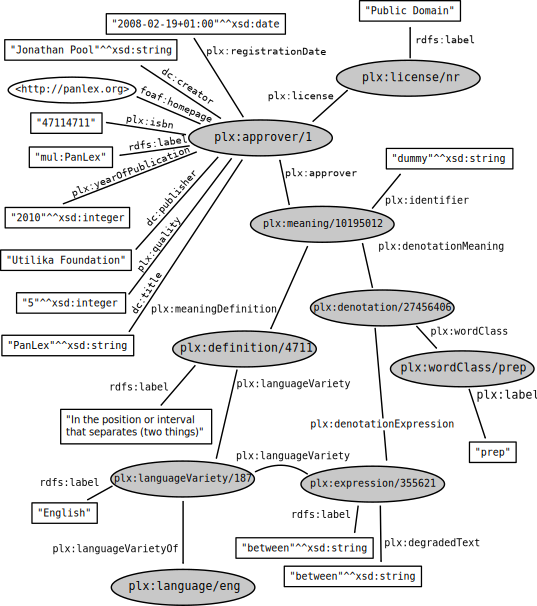
\includegraphics[width=0.46\textwidth]{images/pdf/ontology.pdf}
\caption{Overview of the PanLex RDF Vocabulary}
\label{fig:vocabulary}
\end{figure}

\begin{table}
  \centering\begin{scriptsize}
  \begin{tabular}{p{48px}p{62px}p{70px}}
    Panlex                  & lemon                       & GOLD \\
    \midrule
    \texttt{plx:Denotation} & --                          & \texttt{gold:LinguisticSign} \\
    \texttt{plx:Meaning}    & \texttt{lemon:LexicalSense} & \texttt{gold:SemanticUnit} \\
    \texttt{plx:Expression} & \texttt{lemon:LexicalEntry} & \texttt{gold:FormUnit} \\
  \end{tabular}
  \end{scriptsize}
  \caption{Classes considered to be similar across the re-used vocabulary}
  \label{tbl:sameclasses}
\end{table}

\subsection{Vocabulary Reuse}
\label{sec:vocabulary-reuse}
The PanLex vocabulary is based on PanLex's conceptual schema and
enables all of PanLex's data to be directly exposed as RDF.
%Apart from modeling a PanLex RDF vocabulary
Additionally, we also re-use existing vocuabularies, namely
the \emph{Lexicon Model for Ontologies} (lemon)~\cite{lemon2011} as well as the \emph{General Ontology for Linguistic Description} (GOLD)~\cite{farr2003}.
Since these models differ from the PanLex one, we follow an
incremental approach of aligning the PanLex data with them.
%accordingly. 
% one differ to some
%extend, not the whole schemas were implemented.
\autoref{tbl:sameclasses} shows PanLex classes with their current counterparts
in lemon and GOLD respectively.
The parts implemented in our RDF conversion are displayed in \autoref{fig:goldlemonimplemented}.
\begin{figure}
  \centering
  \includegraphics[width=\linewidth]{images/pdf/gold_lemon_implemented.pdf}
  \caption{Parts of the GOLD (left) and lemon model (right) re-used in PanLex (URI prefixes are omitted for brevity)}
  \label{fig:goldlemonimplemented}
\end{figure}

\subsection{RDF Transformation Workflow}
\label{sec:conversion}
Since new sources are added to the PanLex database on almost a daily basis and because of its current size (\textasciitilde18 GB), the recurrent conversion of the database to capture changes in it is impractical.
%Using conventional hardware, a full conversion takes infeasibly long.
%This makes the testing and debugging of the modeled vocabularies and data very
% time-consuming.
As the PanLex data already reside in a relational database, the use of a virtual RDB2RDF\footnote{\url{http://www.w3.org/2001/sw/wiki/RDB2RDF}} mapping solution is a natural choice.
The \emph{Sparqlify system}\footnote{\url{https://github.com/AKSW/Sparqlify}} offers, besides an efficient query rewriting engine, also a very easy-to-use mapping language, called \emph{Sparqlification Mapping Language} (SML).
Essentially, these mappings consist of three clauses:
The \emph{From} clause specifies the logical SQL table (i.e. table, view, or
query) to be used in the SML view.
The \emph{With} clause binds a set of SPARQL variables to expressions that
yield RDF terms from relational columns.
Finally, the \emph{Construct} clause holds a set of triple patterns.
%clause making use of the defined SPARQL variable definitions.
\autoref{fig:ex:sparqlify-ml} shows an example of an SML view for the
languages in PanLex: From each row of the table \emph{i1} three resources are
created based on the \emph{iso3} column and 
bound to the variable names \emph{?lang}, \emph{?iso3} and \emph{?lexvo3}.
Resources for \emph{?lang} become typed as a \emph{Language} in the PanLex and the \emph{schema.org} namespace.
This view-based approach makes it easy to perform future revisions of RDF mapping, such as
adding support for new vocabularies.
%, as this does not require an extract transform load (ETL) process.
%and can therefore be done with little effort.
%This view-based approach makes it easy to revise the RDF mapping, such as adding support for new vocabular

\begin{figure}
\centering
\begin{lstlisting}
Create View i1 As Construct {
    ?lang a plx:Language, <http://schema.org/Language> ;
          plx:iso639-3Code ?iso3 .
    ?iso3 a plx:Iso639-3Code ;
          owl:sameAs ?lexvo3 .  }
  With
      ?lang = uri(plx:language, '/', ?iso3)
      ?iso3 = uri(plx:iso639-3, '/', ?iso3)
      ?lexvo3 = uri('http://lexvo.org/id/iso639-3/', ?iso3)
  From [[SELECT iso3 FROM i1]]
\end{lstlisting}
\caption{An excerpt of an SML view definition for PanLex's languages. This
example also demonstrates how ``is-a'' relations to schema.org and links to Lexvo are established.}
\label{fig:ex:sparqlify-ml}
\end{figure}

\section{Linking}
\label{sec:linking}
The SML view in (\autoref{fig:ex:sparqlify-ml}) already establishes the interlinking of the PanLex languages with Lexvo.
In this section, we outline the interlinking with DBpedia, where we were interested in creating \emph{valid} and \emph{dereferenceable} links.
Therefore, we iterated the \emph{titles} datasets\footnote{\url{http://wiki.dbpedia.org/Downloads38}}, which map (non-localized) DBpedia URIs to their page titles in the respective language.
For each language version we normalized the labels by applying Unicode NFKD\footnote{\url{http://unicode.org/reports/tr15/}} normalization and removal of punctuation characters.
Each DBpedia resource was then mapped to the PanLex expression that was equal to the resource's normalized label in the respective language.
\autoref{fig:plx-dbp-link-counts} summarizes the number of links obtained.

In total, about 2.5 million links were obtained for approx. 20 million expressions.
This relatively low coverage can be attributed to frequently appearing multi-word expressions that do not match the DBpedia titles well, and the fact that in this work we yet only considered DBpedia datasets for mainstream languages, whereas PanLex focuses on low-density ones.

\begin{table}
  \centering\begin{scriptsize}

  \begin{tabular}{lrclr}
    Language   &   Links   && Language  & Links     \\
    \cline{1-2}\cline{4-5}
    English    & 1,415,241 && Catalan   &    27,779 \\
    German     &   224,146 && Korean    &    24,912 \\
    French     &   187,364 && Turkish   &    22,258 \\
    Italian    &   147,485 && Bulgarian &    19,431 \\
    Spanish    &   117,056 && Hungarian &    18,203 \\
    Portuguese &   112,266 && Slovene   &    11,981 \\
    Polish     &   110,974 && Greek     &     1,112 \\
    \cline{4-5}
    Russian    &    68,040 \\
    Czech      &    28,767 && Total     & 2,537,015 \\
  \end{tabular}
  \end{scriptsize}
  \caption{Number of DBpedia links per language}
  \label{fig:plx-dbp-link-counts}
\end{table}

\section{Publishing}
\label{sec:publishing}
With our RDF conversion work, we complement existing
APIs\footnote{\url{http://panlex.org/try/}} with Linked Data, powered by
Pubby\footnote{\url{http://wifo5-03.informatik.uni-mannheim.de/pubby/}},
and two SPARQL
endpoints\footnote{\url{http://ld.panlex.org/vsparql}}
\footnote{\url{http://ld.panlex.org/sparql}}, ran by Sparqlify and Virtuoso.
% and \url{http://ld.panlex.org/snorql}}.
An overview is shown in ~\autoref{fig:panlex-architecture}.
The SPARQL browser
\emph{SNORQL}\footnote{\url{https://github.com/kurtjx/SNORQL}} can be accessed
by replacing \emph{sparql} with \emph{snorql} in the respective links. Our SML
views and the interlinking code are hosted on GitHub\footnote{\url{https://github.com/AKSW/PanLex-2-RDF}}.
The created linksets are hosted in the PanLex database and are published together with the other data using Sparqlify.
Finally, we offer downloads tagged with timestamps of their creation\footnote{\url{http://ld.panlex.org/downloads/releases/}}.
\begin{figure}
\centering
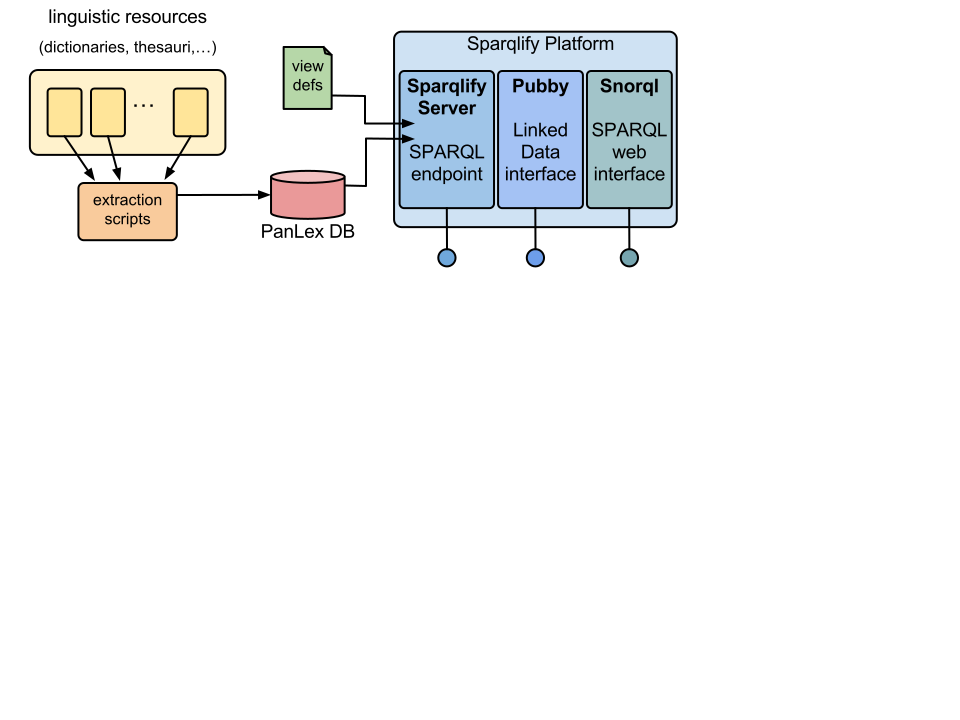
\includegraphics[width=0.5\textwidth]{images/pdf/sparqlify_setup02.pdf}
\caption{PanLex architecture}
\label{fig:panlex-architecture}
\end{figure}

\section{Dataset Benefits and Usage Scenarios}
\label{sec:usage}
There are general benefits of using Semantic Web technologies, such as the
potential for simplified data integration due to RDF and vocabulary reuse, the
possibility of enriching data based on interlinking, drawing advantage from
reasoning and the exploration of the data through the use of generic Semantic
Web tools.
Moreover, some applications, like the TeraDict translation lookup
service\footnote{\url{http://panlex.org/teradict/?lg=eng}}, can now be realized
using SPARQL queries and so easily integrated in other applications.
Due to space considerations, we refer the reader to the PanLex Linked Data
landing page\footnote{\url{http://ld.panlex.org}}, where a
collection of SPARQL queries is maintained.
Also, since PanLex covers a niche of providing linguistic data for
non-mainstream languages, investigation of its fitness for use in cross
language information retrieval, as well as annotation projects, like DBpedia
Spotlight\footnote{\url{http://spotlight.dbpedia.org}}, seems worthwhile.

%exploiting data of projects like Wordnet, e.g. via the LemonWordNet
% dataset\footnote{\url{http://datahub.io/de/dataset/lemonwordnet}} can help
 % finding errors or derive new data and improve translations.
%Another source that could be combined with the PanLex data is the Wortschatz project\footnote{\url{http://wortschatz.uni-leipzig.de/}}.
%Using Wortschatz's co-occurrences statistics of words in different languages one could also improve the recall of word-by-word translations.

%(see \autoref{lst:terradict} for an example).

%that currently only support mainstream languages.
%Apart from this users can easily explore the PanLex data using the
%Linked Data and SPARQL services.
%This also increases the chance of development of new interesting mashups.
% vision web of data
%% \begin{figure}
%% \centering
%% \begin{lstlisting}
%% SELECT ?expr_lbl WHERE {
%%     ?expr_lang rdfs:label "language" .
%%     ?denotation_lang plx:denotationExpression ?expr_lang .
%%     ?denotation_lang plx:denotationMeaning ?meaning .
%%     ?denotation_other plx:denotationMeaning ?meaning .
%%     ?denotation_other plx:denotationExpression ?expr_other .
%%     ?expr_other rdfs:label ?expr_lbl .
%%     FILTER(?expr_lang != ?expr_other)
%% }
%% \end{lstlisting}
%% \caption{SPARQL query to retrieve all known lexical translations of the given English word \emph{`language'}}
%% \label{lst:terradict}
%% \end{figure}

\section{Related Work}
\label{sec:related}
PanLex is a project whose editors integrate information discovered from many lexical resources.
The extraction of information from linguistic sources, and techniques for automatically inferring translations,
are relevant work discussed in \cite{panlex_probtrans}.
%A similar approach of linking expressions to meanings is followed by the
% \emph{Global Wordnet Association}.
An important related initiative is the Global Wordnet Association (GWA)\footnote{\url{http://www.globalwordnet.org/}\vspace{0.7em}},
which offers a platform for sharing wordnets and, among other goals, uniformly representing wordnets
of different languages and establishing a universal index of meaning.
Wordnets are usually focused on the
definition of \emph{synsets} and relations between them in a single language; GWA is helping to transform these single-language synonym silos into a virtual multilingual translation resource. PanLex is approximating that, in a different way, by integrating data from numerous wordnets along with translingual sources into a single graph.
%As already mentioned in PanLex there can be several meaning entities
% representing the same unique sense.
In the Semantic Web context, several standard or quasi-standard vocabularies and ontologies have been developed with the rise of the \emph{Linguistic Linked Open Data} movement.
Examples include the
\emph{Ontologies of Linguistic Annotation} (OLiA)~\cite{olia2010} for modeling
lexicon and machine-readable dictionaries, \emph{POWLA} for modeling linguistic corpora\cite{powla2012} and the \emph{Natural Language Processing Interchange Format} (NIF)\footnote{\url{http://nlp2rdf.org/nif-1-0}}.

\section{Conclusions and Future Work}
\label{sec:conclusion}
In this dataset description we detailed the PanLex database and its conversion to RDF.
Based on our URI and vocabulary design, we created appropriate view definitions
for the \emph{Sparqlify} system, which carries out the actual RDF
transformation.
Furthermore, we interlinked the languages in PanLex with Lexvo, and created about 2.5 million links to DBpedia for expressions in 16 languages.
With the integration of lemon and GOLD we also support data access via external linguistic ontologies.

We intend to address some limitations in the future:
The relations among PanLex's information sources, if treated as distinct datasets, could be modeled with the VoID vocabulary\footnote{\url{http://rdfs.org/ns/void}}.
The source entity should be refactored to reference users and information sources as distinct entities.
%Attribution is currently limited to (assertion) sources,
% obscuring the possible roles of multiple editors in iteratively interpreting sources and the subsidiary sources of data in sources that are %themselves aggregations.
Metadata attached to PanLex denotations are currently limited to arbitrary pairs of strings,
but this sacrifices discovery possibilities when the metadata
%(as they often do)
describe facts that can again be expressed with PanLex expressions.
% (e.g., that the expression is archaic).
Finally, new collaborations between PanLex and related fields (e.g. as language identification, language geolocation, lemmatization, transliteration, localization, etc.) are promising arenas for development.

\bibliographystyle{abbrv}
\bibliography{bibliography,../../bib/aksw}

\end{document}
